If we look at the criteria that defines life it could be that our surroundings is part of a life form.
This has lead people to make different theories, and even predictions that humans one day will be able to produce intelligent beings.

\subsubsection*{The Gaia theory}
One of the more interesting theories is Gaia theory \cite{Lovelock}, which relates to life on micro and macro scales. Now this is a theory, but it's an interesting one, and it's worth noting, especially with what we now know of the unwitting coordination of the cells in our body.
Gaia theory, originally concocted by a chemist named James Lovelock in the 60's, is about how the very planet we live on can be, just as we are, a single organism consisting of trillions of lifeforms working together, unwittingly.
Could it be that we are just cells in the body of the planet Earth?
Are we zooming around the sun in a single organic spaceship?
Could we, in the future, as our space travel talents grow, encounter living planets as singular entities?

%\subsubsection*{The universe is alive}
\subsection{Multiverses}
\initial{I}f you put the most vivid part of your brain in action, there are really no limits on how abstract one can make the concept of life.
Why must \textit{life} be restricted to something close to our own size?
Why must \textit{life} be restricted to something that resembles us at all?
We have mentioned the Gaia theory, but why stop there?
The Universe itself could also be considered a living organism, if what some theoretical physicists believe are true.
This is where we introduce the idea of a multiverse.

The idea goes as follows:
What if there is more than one universe?
What if these are all connected to each other in a dimension completely oblivious to us?
What if universes could create new universes?

\begin{center}
	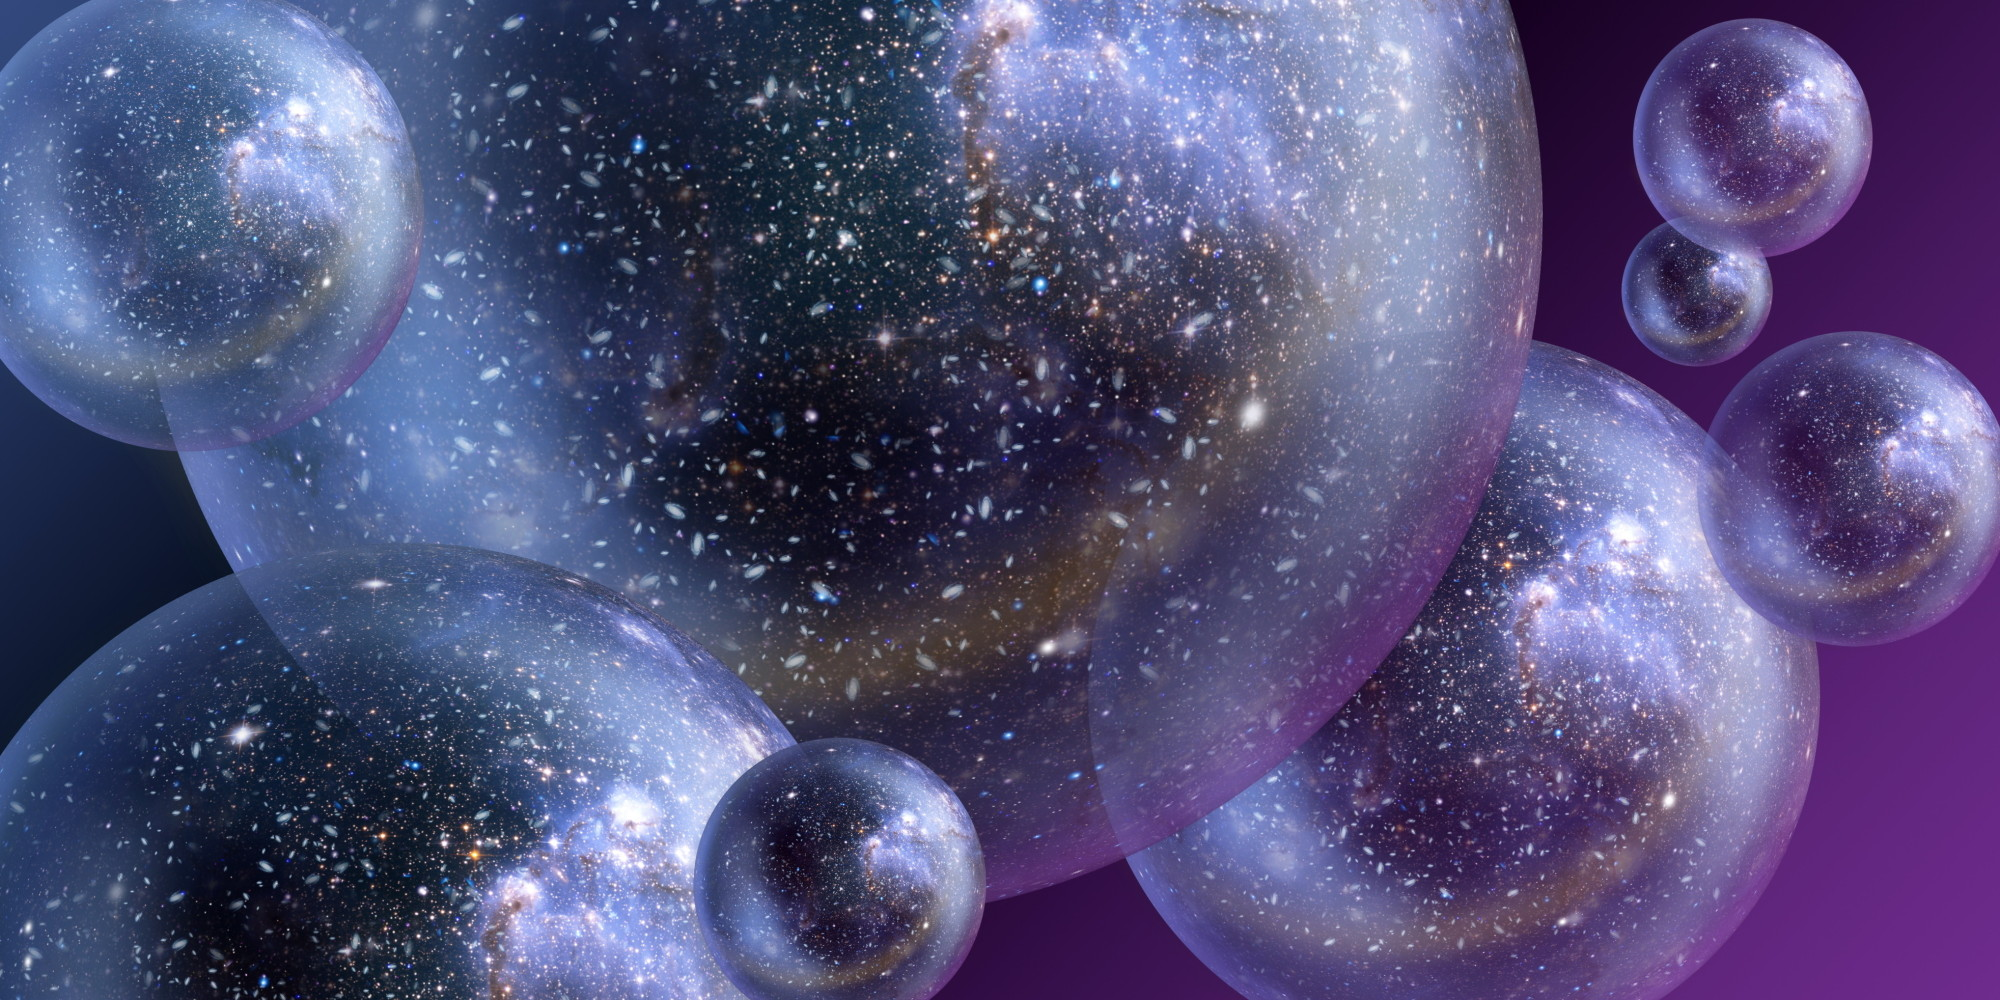
\includegraphics[width=0.47\textwidth]{multiverse.jpg}
\end{center}
%http://i.huffpost.com/gen/2229248/images/o-PARALLEL-UNIVERSES-facebook.jpg

Multiverse has been suggested several times in science fiction, often in context of time travel or alternate universes.
Time travel would for example, split the history into two different universes.
One where the time travel never happened and one where it did.
Alternate universes would often be a thought experiment where you could have been born in a different place and time, but still be \textit{you}.
Could there be a world out there where you are the President of the United States?

There also exists a more scientific, or less fictional, version of this idea.
In short, different universes would have different physical conditions, and all of them would pan out differently one from another.
The beginning of a universe would be something like the Big Bang.
From there it grows and changes, governed by its own physical laws and constants.
In time it may come to a stage where it creates black holes.
Some think this is how a universe might reproduce.
The newly formed universe would have slightly different attributes than its parent.
Some universes may die, some may have physical conditions that keep them in an endless cycle of expanding and retracting.

Universes could undergo birth, growth and death.
They evolve throughout their generations with every infant universe being slightly different from its parent.
Only the ones capable of creating black holes will be \textit{successful}.
How these organisms could feed and move in higher dimensions is even more vivid and far fetched.
After all, this is only an idea.
At least for now.

\subsubsection*{Life in a computer}
The interest in Artificial Intelligence (AI) has risen in recent years, as business corporations see the opportunity to replace human manpower with computers to enable increased workloads.
Development in this field of study has of course lead to some interesting inventions.
In early 2014 Facebook announced that their face recognition software was as accurate as the human brain \cite{facebook}.
This example shows how inventions in AI have a rather practical approach these days, with single purposes, although the holy grail would be to create a more complex software and even with consciousness.
If algorithms like the one of Facebook's were to be simplified or when their patents are no longer valid, perhaps even more complex algorithms can be formed.

AI is based on human behaviour and is also connected to psychology.
The assumption that humans are the most intelligent beings gives us the motivation to try to replicate ourselves.
Despite what many people believe, AI does not have to include fancy robotics and machinery, nor does it have to be an android in physical matters.
An agent; which is the smallest unit of AI, senses, reflects and actuates, where the sensors and actuators gives its physical constraints, and the reflection is core of the AI.
There are two levels of AI, weak AI and strong AI. Weak AI is when an agent acts intelligent, which disables a Turing test to distinguish it from a human.
When it comes to an intelligent agent, it is a subject to strong AI, however this is yet to be made.